% ------------------------------------------------------------------------------
% includes preamble stuff
\documentclass[a4paper,11pt]{report}
%\documentclass[a4paper,11pt]{article}

% sans serif font 
%\renewcommand{\familydefault}{\sfdefault}


%title page stuff
\newcommand{\HRule}{\rule{\linewidth}{0.5mm}}

% margins
\usepackage[top=2.5cm, bottom=2.5cm, left=4cm, right=2.5cm]{geometry}
\geometry{a4paper} % or letterpaper (US) or a5paper or....
%\geometry{margin=1in}

\usepackage{fancyhdr}
\pagestyle{fancyplain}
\fancyfoot[C]{\thepage}                 % page number in centre of foot.
\fancyfoot[R]{\small{M. J. Hawes, 10238908}}	% right of footer. 
\rhead{}

% \usepackage{setspace}           
% \onehalfspacing               % Sets the line spacing to 1.5


% ------------------------------------------------------------------------------
% provides comment functionality
\usepackage{verbatim}

% ------------------------------------------------------------------------------
% setting up harvard style refs
%\usepackage{harvard}
%\bibliographystyle{harvard}
\bibliographystyle{plain}

\usepackage{cite}

% ------------------------------------------------------------------------------
% needed for code listings
\usepackage{color}
\usepackage{xcolor}
\usepackage{listings}

\usepackage{caption}
\DeclareCaptionFont{black}{\color{black}}
\DeclareCaptionFormat{listing}{\colorbox{white}{\parbox{\textwidth}{#1#2#3}}}
\captionsetup[lstlisting]{format=listing,labelfont=black,textfont=black}

\lstset{ %
language=C,                % choose the language of the code
basicstyle=\footnotesize,       % the size of the fonts that are used for the code
numbers=left,                   % where to put the line-numbers
numberstyle=\footnotesize,      % the size of the fonts that are used for the line-numbers
stepnumber=1,                   % the step between two line-numbers. If it is 1 each line will be numbered
numbersep=5pt,                  % how far the line-numbers are from the code
backgroundcolor=\color{black!6!white},  % choose the background color. You must add \usepackage{color}
showspaces=false,               % show spaces adding particular underscores
showstringspaces=false,         % underline spaces within strings
showtabs=false,                 % show tabs within strings adding particular underscores
frame=single,           % adds a frame around the code
tabsize=2,          % sets default tabsize to 2 spaces
captionpos=b,           % sets the caption-position to bottom
breaklines=true,        % sets automatic line breaking
breakatwhitespace=true,    % sets if automatic breaks should only happen at whitespace
%escapeinside={\%*}{*)}          % if you want to add a comment within your code
}

% ------------------------------------------------------------------------------
% Graphics stuff for images
\usepackage{graphicx}
\DeclareGraphicsExtensions{.jpg,.jpeg,.png}
\graphicspath{ {./imgs/} }

% for graphs
\usepackage{tikz}
\usepackage{pgfplots}

\usepackage{epstopdf}		% .eps to .pdf

\usepackage{float}
%\floatstyle{boxed}
\restylefloat{figure}
\usepackage{caption}
\usepackage{subcaption}

\renewcommand{\thesubfigure}{\roman{subfigure}}
\captionsetup[subfigure]{labelformat=simple, labelsep=colon}

% Caption stuff
\begin{comment}
\DeclareCaptionFormat{myformat}{%
  \colorbox{lightgray!30}{\parbox{\dimexpr\textwidth-2\fboxsep-2\fboxrule\relax}{#1#2#3}}
} 
\captionsetup[figure]{format=myformat}
\captionsetup[lstlisting]{format=myformat}
\captionsetup[table]{format=myformat}
\end{comment}

% ------------------------------------------------------------------------------
% Maths packages
\usepackage{amsmath}

% ------------------------------------------------------------------------------
% Glossary packages
\newcommand*{\glossfirstformat}[1]{\textbf{#1}}

\usepackage[]{glossaries}
\renewcommand*{\glspostdescription}{}
\glossarystyle{list}
\makeglossaries

\renewcommand{\glsdisplayfirst}[4]{\glossfirstformat{#1#4}}
\renewcommand*{\glsnamefont}{\sffamily}
\renewcommand*{\glossarymark}[1]{}

\newglossaryentry{Makefile}
{
    name={Makefile},
    description={},
    plural={Makefiles}
}

\newglossaryentry{thread}
{
    name={thread},
    description={},
    plural={threads}
}

\newglossaryentry{multi-threaded algorithm}
{
    name={multi-threaded algorithm},
    description={},
    plural={multi-threaded algorithms}
}

\newglossaryentry{scheduling}
{
    name={scheduling},
    description={},    
}

\newglossaryentry{worker-thread}
{
    name={worker-thread},
    description={},
    plural={worker-threads}
}

\newglossaryentry{monitor-thread}
{
    name={monitor-thread},
    description={},
    plural={monitor-threads}
}

\newglossaryentry{mutex}
{
    name={mutex},
    description={},
    plural={mutexes}
}

\newglossaryentry{barrier}
{
    name={barrier},
    description={},
    plural={barriers}
}

\newglossaryentry{conditional-variable}
{
    name={conditional-variable},
    description={},
    plural={conditional-variables}
}
\newglossaryentry{load-balancing}
{
    name={load-balancing},
    description={},
}

\newglossaryentry{work-stealing}
{
    name={work-stealing},
    description={A processor which is starved of work attempts to ``steal'' 
                 work from other processors},
}

\newglossaryentry{thief}
{
    name={thief},
    description={},
    plural={thieves}
}

\newglossaryentry{victim}
{
    name={victim},
    description={},
    plural={victims}
}

\newglossaryentry{ready-deque}
{
    name={ready-deque},
    description={},
    plural={ready-deques}
}

\newglossaryentry{non-blocking}
{
    name={non-blocking},
    description={},
}

\newglossaryentry{steal-operation}
{
    name={steal-operation},
    description={},
}

\newglossaryentry{work-sharing}
{
    name={work-stealing},
    description={A processor which creates new work attempts to migrate it to 
                 another underutilised processor at creation time},
}

\newglossaryentry{locality}
{
    name={locality},
    description={},
}

\newglossaryentry{julia-set}
{
    name={julia-set},
    description={},
    plural={julia-sets}
}

\newglossaryentry{filled julia-set}
{
    name={filled julia-set},
    description={},
    plural={filled julia-sets}
}

\newglossaryentry{critical-orbit}
{
    name={critical-orbit},
    description={},
    plural={critical-orbits}
}

\newglossaryentry{fractal}
{
    name={fractal},
    description={},
    plural={fractals}
}

\newglossaryentry{complex-number}
{
    name={complex-numer},
    description={},
    plural={complex-numbers}
}

\newglossaryentry{real-world-fractal}
{
    name={real-world-fractal},
    description={},
    plural={real-world-fractals}
}

\newglossaryentry{mathematical-fractal}
{
    name={mathematical-fractal},
    description={},
    plural={mathematical-fractals}
}

\newglossaryentry{scale-invariance}
{
    name={scale-invariance},
    description={},
}

\newglossaryentry{self-similarity}
{
    name={self-similarity},
    description={},
}

\newglossaryentry{exact self-similarity}
{
    name={exact self-similarity},
    description={},
}

\newglossaryentry{quasi self-similarity}
{
    name={quasi self-similarity},
    description={},
    plural={quasi self-similar}
}



% ------------------------------------------------------------------------------
% Appendix packages
\usepackage[toc,page]{appendix}

\makeatletter
    \def\thebibliography#1{\chapter*{References\@mkboth
      {REFERENCES}{REFERENCES}}\list
      {[\arabic{enumi}]}{\settowidth\labelwidth{[#1]}\leftmargin\labelwidth
	\advance\leftmargin\labelsep
	\usecounter{enumi}}
	\def\newblock{\hskip .11em plus .33em minus .07em}
	\sloppy\clubpenalty4000\widowpenalty4000
	\sfcode`\.=1000\relax}
    \makeatother


% ------------------------------------------------------------------------------
%title
\title{
\huge A Work-Stealing Scheduling Technique Applied to Computing the Mandelbrot Set.
}

\author{
  Martin J Hawes\\
  \\
  Department of Computer Science, \\
  The University of Hertfordshire \\ 
  \\
  \textit{hawesmartin@googlemail.com}\\
}

% ------------------------------------------------------------------------------
% - Document starts here
% ------------------------------------------------------------------------------

\begin{document}
\maketitle
\date{}

% ---------------------------------------------------------------------------------------------------------------------------------------------------------------
\pagenumbering{Roman}
\section*{Abstract}


% ---------------------------------------------------------------------------------------------------------------------------------------------------------------
\section*{Acknowledgements}


% ---------------------------------------------------------------------------------------------------------------------------------------------------------------
\clearpage
\pagenumbering{arabic}
\setcounter{page}{1}
\tableofcontents

% ---------------------------------------------------------------------------------------------------------------------------------------------------------------
% ---------------------------------------------------------------------------------------------------------------------------------------------------------------
% ---------------------------------------------------------------------------------------------------------------------------------------------------------------
\chapter{Introduction}

% ---------------------------------------------------------------------------------------------------------------------------------------------------------------
% ---------------------------------------------------------------------------------------------------------------------------------------------------------------
% ---------------------------------------------------------------------------------------------------------------------------------------------------------------
\chapter{Background Research}
% ---------------------------------------------------------------------------------------------------------------------------------------------------------------
% NO-CITES
%\nocite{jmcguin}
%-------------

\section{Scheduling Techniques for Multi-Threaded Computations}
This section briefly describes the problems associated with scheduling Multi-Threaded Algorithms and 
the major paradigms that have surfaced.

% explain problems here...... is this better off in the intro??
In order to efficiently utilize a parallel computer architecture it is desirable to minimize
the amount of time a processor spends idle or performing other logistical tasks, I.e not doing work. 
When a computation's \textit{concurrent sub-tasks} or \textit{threads} incur a regular cost in processor
time, each processor can simply have the same amount of work assigned to them. When the computation has
more irregular or dynamically growing sub-tasks a problem arises resulting in 
processors becoming idle while others still remain working. The solution to this problem is refereed to as
\textit{load balancing} and can be described as a form of dynamic scheduling that ensures each processor 
spends approximately the same amount of time working. This means processors generally spend
less time idle, however have to deal with scheduling overheads as a trade-off.

When considering the scheduling of multi-threaded computations, two major load balancing techniques have been used.
These are \textit{work-sharing} and \textit{work-stealing}.

\begin{itemize}
\item \textbf{Work-Sharing:} A processor which creates new work attempts to migrate it to another underutilised processor at creation time. 
\item \textbf{Work-Stealing:} A processor that is starved of work attempts to ``steal'' work from other processors. 
\end{itemize}

Both techniques intend to promote balanced work-load across all processors, however in Work-Stealing
the frequency of work migrations is lower. When all processors have a 
high work-load and no need to ``steal" this becomes useful because threads need not get 
migrated at all. With work-sharing work migration occurs each time new work is created \cite[p.~2]{blumleis}.
This also suggests that work-stealing promotes better locality and grouping of sub-tasks, as spawned work 
stays with the same processor until stolen.


% ---------------------------------------------------------------------------------------------------------------------------------------------------------------
\section{The Work-Stealing Technique - Described in Depth}

% explain approaches put forward by various papers. Explain J McGuiness' mandelbrot specific approach last.

% ---------------------------------------------------------------------------------------------------------------------------------------------------------------
\section{The Mandelbrot Set}

%\subsection{Background}
The Mandelbrot set is a set of complex numbers which when plotted produce a spectacular and recognisable shape as illustrated in figure~\ref{fig:mandelimg}.
It is often presented as a colourful and striking image and has been described by some as the most beautiful object in all of mathematics \cite[p.~234]{chaosfract}.
The complex numbers that comprise the set are closely related to \textit{Julia Sets}. 
In-fact the Mandelbrot set can be described as a catalogue of Julia Sets which, when plotted, all points are \textit{connected}, 
forming a \textit{single, unbroken shape} \cite[p.~177]{fractimg}.

The set is named for the mathematician \textit{Benoit Mandelbrot}, who discovered it in 1980 \cite{fracnature , fractimg}. He was a pioneer in the study of 
fractal geometry and also coined the term \textit{fractal}, of which both the Mandelbrot set, and Julia sets are examples of. 

In this section I will give a more detailed explanation of the areas mentioned here. 

\begin{figure}[t]
  \caption{A rendering of The Mandelbrot Set generated using the program ``fraqtive"\cite{fraqtive}.}
  \label{fig:mandelimg}
  \centering
    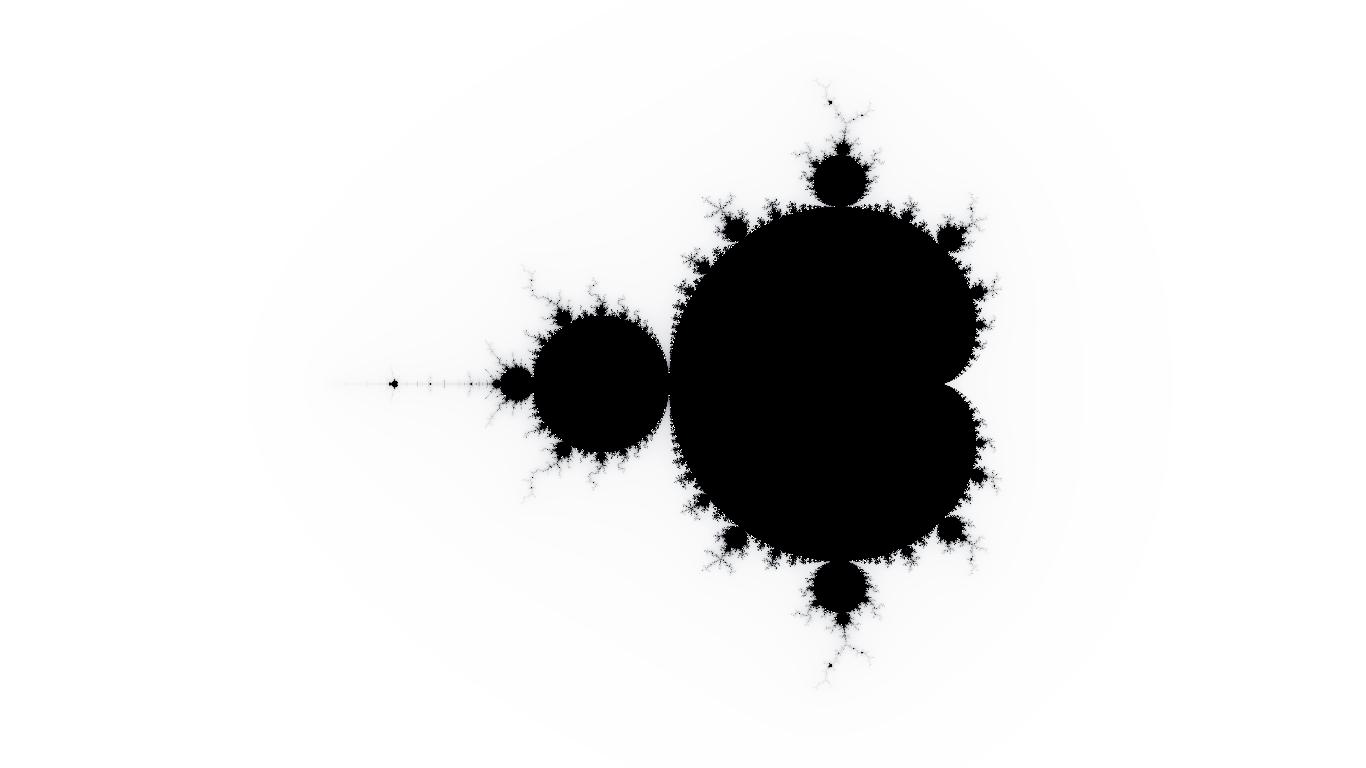
\includegraphics[width=1\textwidth]{mandelbrot}
\end{figure}

\subsection*{Fractals and Self-Similarity} 
%TODO: this section needs citations all over the shop!
A fractal is a means of describing shapes which are more complex than classical geometric shapes. The leaves of a pine tree or the forks of a 
lightning bolt are obvious examples of real things that fractals allow us to more faithfully describe. 
These \textit{real world fractals} are similar to \textit{mathematical fractals}, 
of which the Mandelbrot set is an example, but differ in that they do not display the property of \textit{Scale Invariance}. 

Fractals have a fractional dimension. % TODO MORE HERE!!!!!
 
A property of fractals (but not all) is \textit{Self-Similarity}, where the shape is comprised of smaller ``copies" of itself. 
This is known as \textit{Exact Self-Similarity} and means that the shape is identical at any scale.
A well-known example of this is the \textit{Triadic Koch Snowflake} which is a fractal constructed using equilateral triangles. 
It is important to note here that The Mandelbrot set does not quite show the same property, it is said to be 
\textit{Quasi Self-Similar}. This means that the shape is approximately similar at all scales, in that the shape is replicated but in a slightly distorted
form with each ``copy".

It turns out there are many rather useful applications for fractals. To name a few; computer game graphics, %FIND MORE EXAMPLES WITH CITATIONS.

\subsection*{Julia Sets}

To understand the basis of the Mandelbrot set it is first necessary to understand it's relation to \textit{Julia Sets}.
The function in equation~\ref{eq:julia1} is iterated infinitely where \(c\) is fixed.
The \textit{filled Julia Set} is comprised of all values of \(z_0\) where the result is bounded and does not tend towards infinity.
The \textit{Julia Set} is comprised of those members of the \textit{filled Julia Set} which lie on the boundary \cite{chaosfract}.
In the interest of keeping this report readable, and because filled Julia Sets are more relevant, filled Julia sets will be 
referred to simply as \textit{Julia Sets}.

% express the set notation for f(x) -> infinity.???? TODO
\begin{equation}\label{eq:julia1}
f(z) = z^2 + c
\end{equation}

With regards to the Mandelbrot Set I am interested in Julia Sets in which the values \(c\) and \(x\) used are expressed as a complex number. 
Figure~\ref{fig:juliaimgs} illustrates some examples of such sets. 

\begin{figure}[h]
%\centering
\begin{subfigure}[b]{0.48\textwidth}
  \centering    
  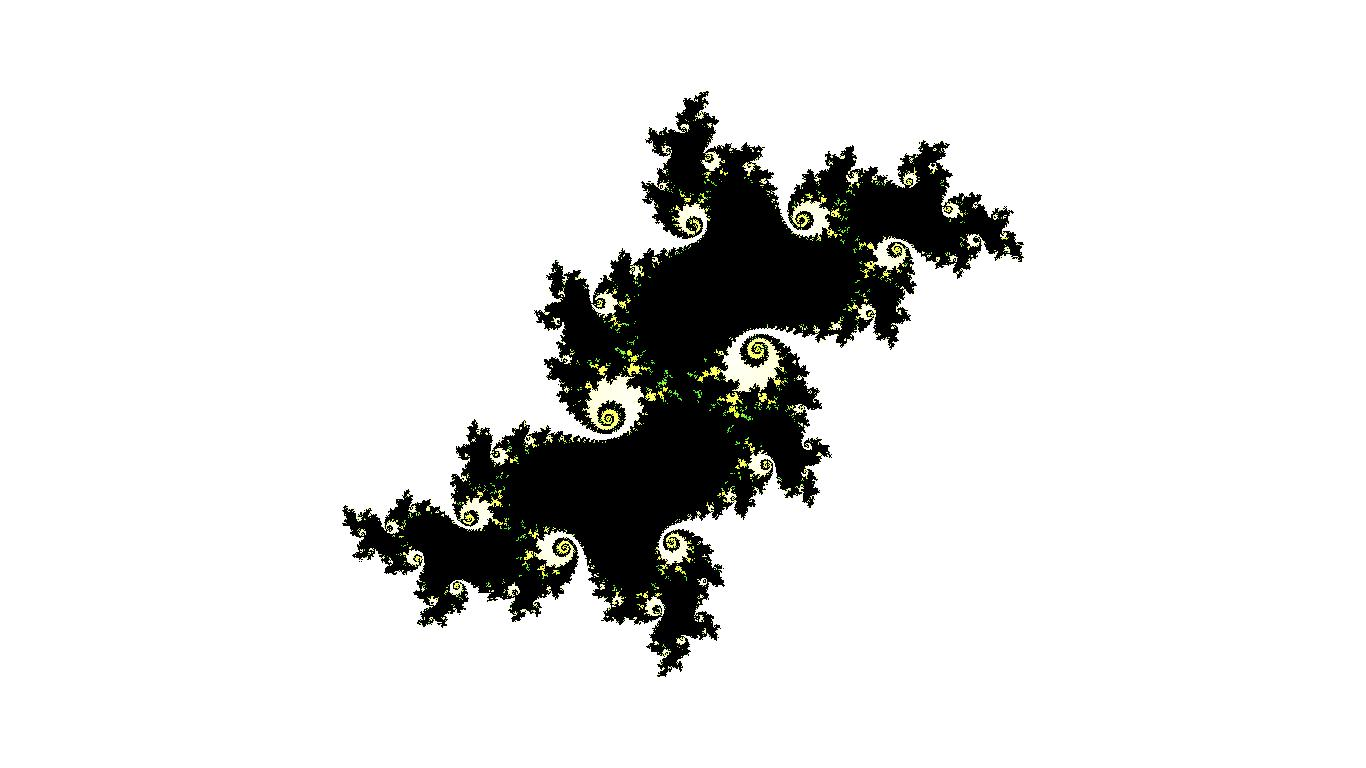
\includegraphics[width=\textwidth]{julia-con}
  \caption{
    \tiny The Julia Set where \(c = -0.1 + 0.649i\)
  }
  \label{fig:juliaimgcon}
\end{subfigure}
~ %spacer
\begin{subfigure}[b]{0.48\textwidth}
  \centering
  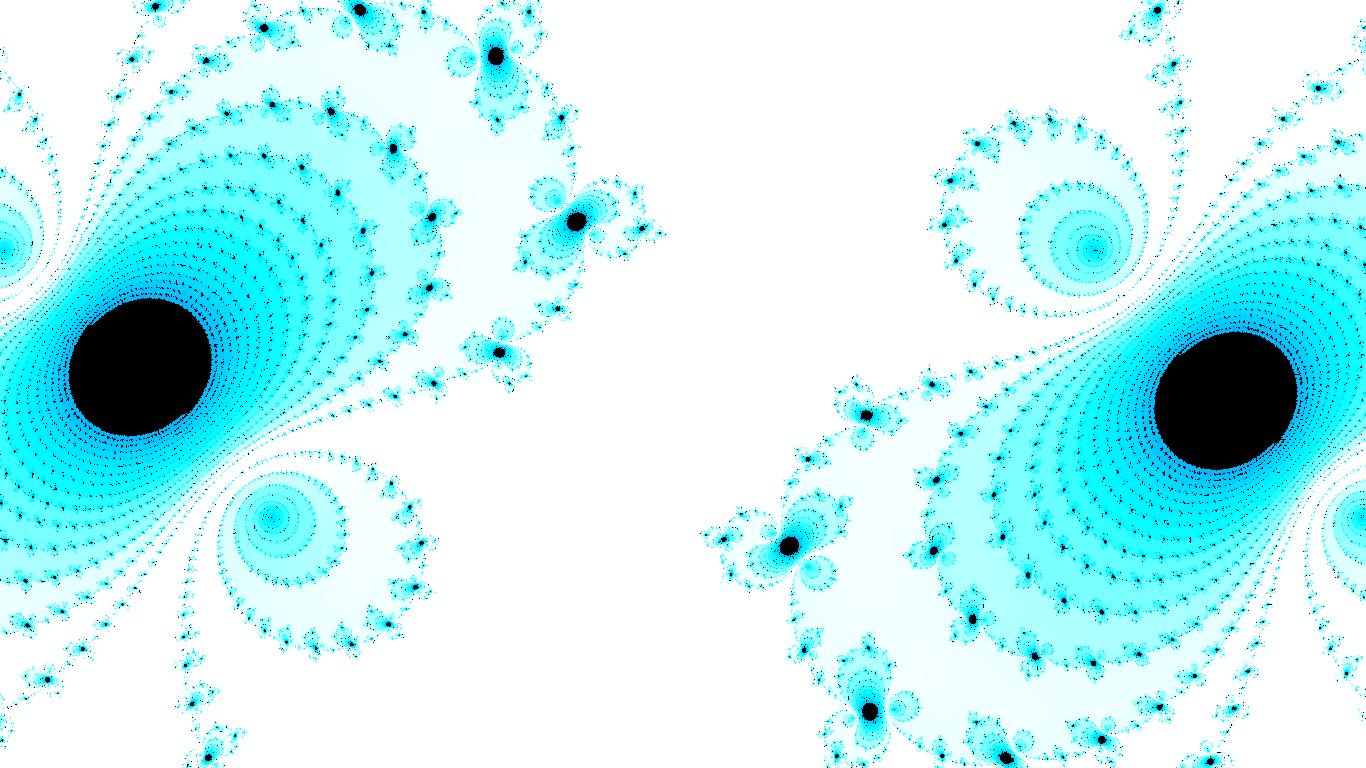
\includegraphics[width=\textwidth]{julia-ncon}
  \caption{
    \tiny The Julia Set where \(c = -0.75 + 0.03i\)
  }
  \label{fig:juliaimgncon}
\end{subfigure}
% full caption
\caption{
  Two Julia Sets rendered using the program \textit{fraqtive}\cite{fraqtive}. 
  Figure~\ref{fig:juliaimgcon} is a member of the Mandelbrot set, 
  figure~\ref{fig:juliaimgncon} is not.
}
\label{fig:juliaimgs}
    %include this because the block is HUGE!!
\centering
\begin{subfigure}[b]{0.48\textwidth}
  \centering    
  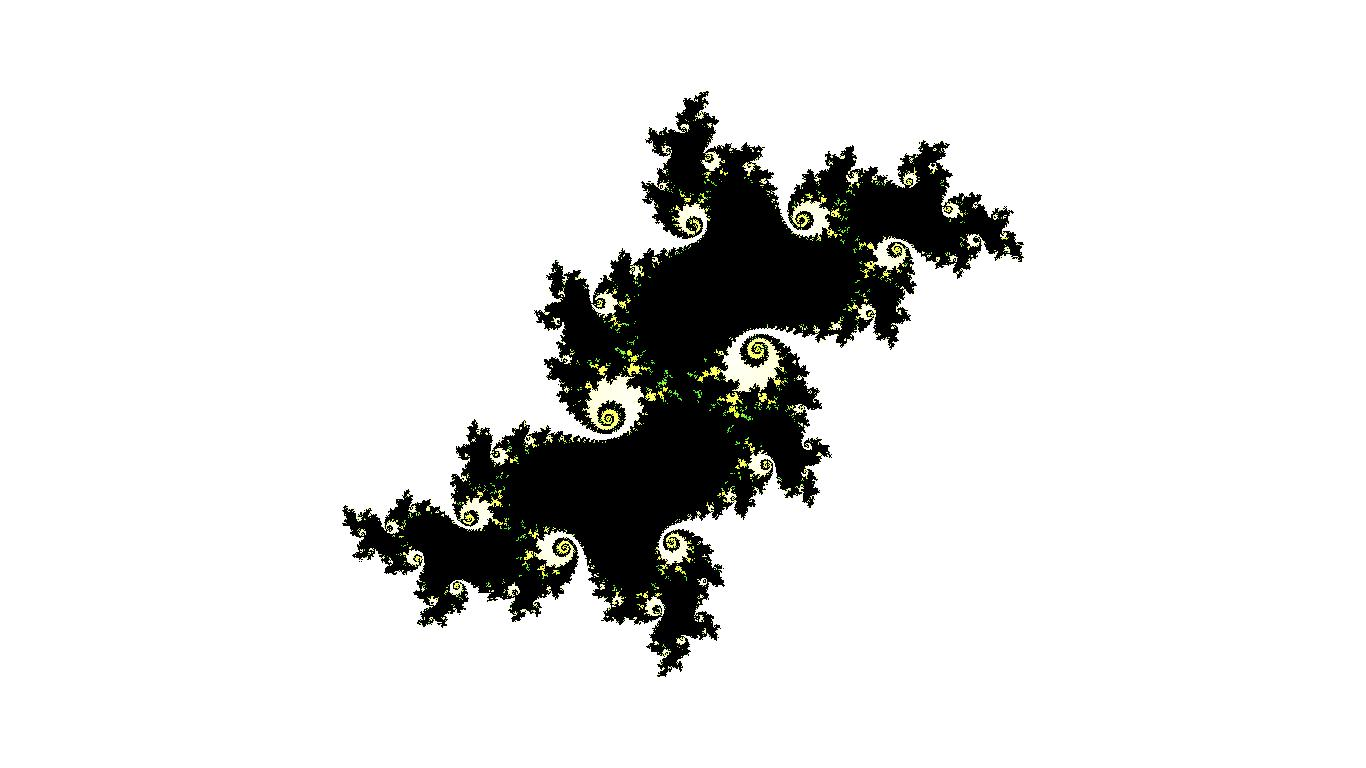
\includegraphics[width=\textwidth]{julia-con}
  \caption{
    \tiny The Julia Set where \(c = -0.1 + 0.649i\)
  }
  \label{fig:juliaimgcon}
\end{subfigure}
~ %spacer
\begin{subfigure}[b]{0.48\textwidth}
  \centering
  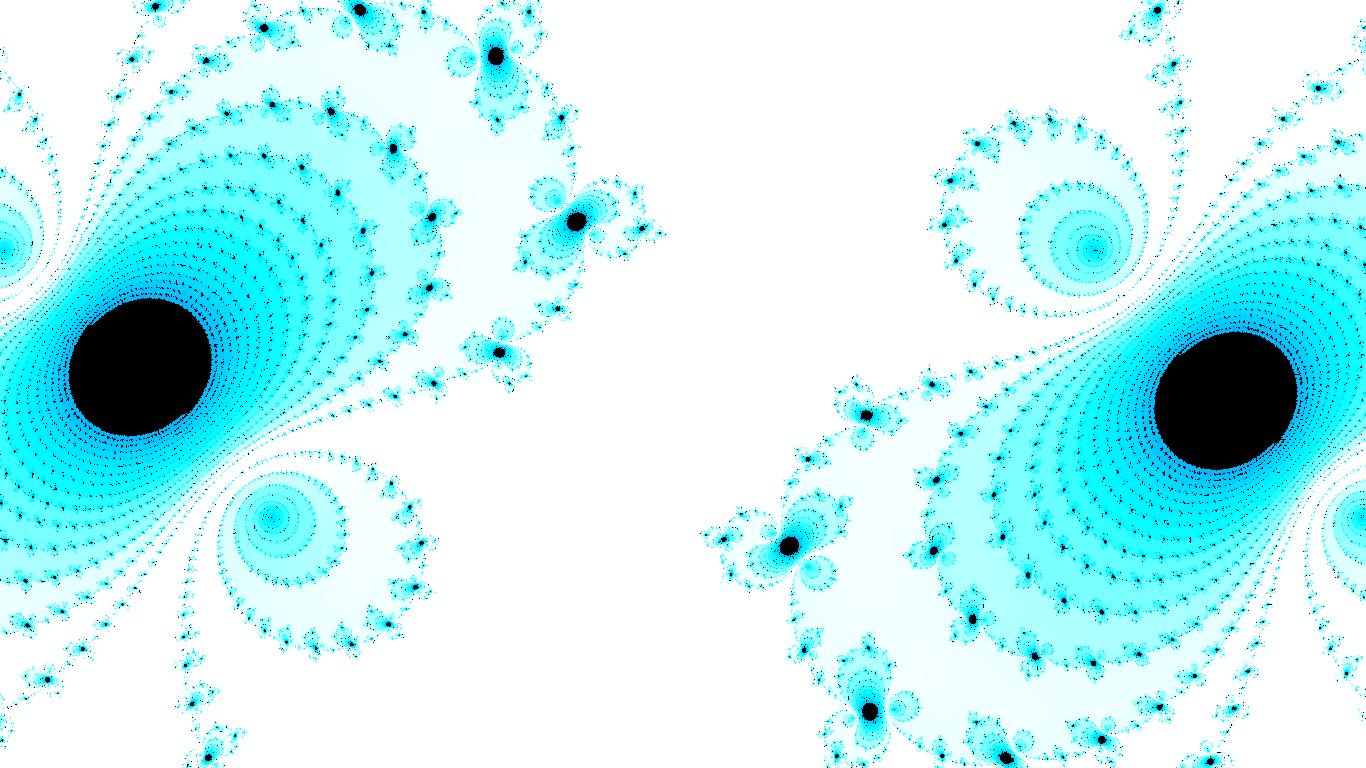
\includegraphics[width=\textwidth]{julia-ncon}
  \caption{
    \tiny The Julia Set where \(c = -0.75 + 0.03i\)
  }
  \label{fig:juliaimgncon}
\end{subfigure}
% full caption
\caption{
  Two Julia Sets rendered using the program \textit{fraqtive}\cite{fraqtive}. 
  Figure~\ref{fig:juliaimgcon} is a member of the Mandelbrot set, 
  figure~\ref{fig:juliaimgncon} is not.
}
\label{fig:juliaimgs}
\end{figure}

\subsection*{Computing the Mandelbrot Set}

The set is comprised of those Julia Sets which are \textit{connected}. In order to determine whether a Julia Set possesses this property,
we need only compute the result for \(z_0\). If this tends towards infinity the value \(c\) is not a member of the Mandelbrot Set. If it 
does not, then it is a member. This is known as the \textit{critical orbit} and is useful because it means we do not have to compute
the entire Julia Set for each value of \(c\).


% ---------------------------------------------------------------------------------------------------------------------------------------------------------------
\section{Programming Tools}

In this section I will discuss some of the programming tools which are candidates
for use in my implementation. 
The tools discussed in this section are all viable options for a Linux platform.

\subsection*{Languages}

\begin{itemize}
\item \textbf{C:} 
\item \textbf{C++:}
\item \textbf{Java:}
\end{itemize}

\subsection*{Concurrent Programming Libraries}
In order to implement Work-Stealing, support for programming threads 
with a suitable level of control is required.

\begin{itemize}
\item \textbf{POSIX Threads (pthreads):} Provides low level manipulation of threads for the C programming language \cite{pthreadover}. 
              It is a library based on IEEE standard 1003.1. Thread programming is achieved through use of a set of functions and data
              structures provided, such as \textit{mutexes}, \textit{semaphores}, \textit{ }. %TODO
             
\item \textbf{Open Multiprocessing (OpenMP):} Provides abstract thread programming interfaces for C, C++, and fortran.
              In general OpenMP only allows coarse grained manipulation of threads through features such as parallel loops %TODO
              \cite{ompvspthr}

\item \textbf{Java Threads:}
\end{itemize}

\subsection*{Graphical Output}
For the purpose of demonstrating that the program correctly generates a raster plane
of the Mandelbrot set, a graphical rendering of the plane will be output.

\begin{itemize}
\item \textbf{PPM Output File:} The simplest option is to output to a Portable Pixel Map (PPM) file. It is 
              text-file based and easy to implement but produces rather large files. 
              The process of outputting to a text file is inherently serial in nature,
              so with large image resolutions processing takes a long time.
              There is support for both grey-scale (Portable Grey-scale Map format) and colour images. 
              \cite{ppmspec}
              
\item \textbf{GNU Plot:} A graph plotting package available for multiple operating systems. 
              Supports screen display or file output of both 2d and 3d graphics \cite{gnuplot}.
              There are programming interfaces available for various languages such as C \cite{gnuplotcint}, C++ \cite{gnuplotcppint}, 
              and Java \cite{gnuplotjint}.
              
%\item \textbf{OpenGL}
\end{itemize}


% ---------------------------------------------------------------------------------------------------------------------------------------------------------------
% ---------------------------------------------------------------------------------------------------------------------------------------------------------------
% ---------------------------------------------------------------------------------------------------------------------------------------------------------------
\chapter{Main Chapters}
% ---------------------------------------------------------------------------------------------------------------------------------------------------------------
\section{Design of the Algorithm}

% ---------------------------------------------------------------------------------------------------------------------------------------------------------------
\section{The Implementation}

% ---------------------------------------------------------------------------------------------------------------------------------------------------------------
\subsection{An Algorithm to Compute the Mandelbrot Set}

% talk about the static keyword in C for the array.
% talk about inlining some functions
% talk about 

% ---------------------------------------------------------------------------------------------------------------------------------------------------------------
\subsection{A Concurrent Algorithm to Compute the Mandelbrot Set}

% ---------------------------------------------------------------------------------------------------------------------------------------------------------------
\section{Features for Demonstration}

% ---------------------------------------------------------------------------------------------------------------------------------------------------------------
\section{Validation and Verification}

% ---------------------------------------------------------------------------------------------------------------------------------------------------------------
% ---------------------------------------------------------------------------------------------------------------------------------------------------------------
% ---------------------------------------------------------------------------------------------------------------------------------------------------------------
\chapter{Discussion and Evaluation}
% ---------------------------------------------------------------------------------------------------------------------------------------------------------------
\section{Analysis of the Algorithm}

% ---------------------------------------------------------------------------------------------------------------------------------------------------------------
\section{Reflection on Project}

% ---------------------------------------------------------------------------------------------------------------------------------------------------------------
% ---------------------------------------------------------------------------------------------------------------------------------------------------------------
% ---------------------------------------------------------------------------------------------------------------------------------------------------------------
\chapter{Resources}

\nocite{*}

% refs\bibs:
\bibliography{refs}

% ---------------------------------------------------------------------------------------------------------------------------------------------------------------
% ---------------------------------------------------------------------------------------------------------------------------------------------------------------
% ---------------------------------------------------------------------------------------------------------------------------------------------------------------
\chapter{Appendices}

\end{document}
